\documentclass[landscape]{article}

\usepackage{graphicx}

\voffset = -90pt
\hoffset = -170pt
\textwidth = 700pt
\textheight = 550pt

\begin{document}

\thispagestyle{empty}

\section*{Design of a Very Simple Game on Paper}

The goal in this game is to go from START to END using the following rules:

\begin{enumerate}

  \item The player begins at ``START'' with five hit points (HP) strength set to
    zero;

  \item The player can move any direction and any number of steps, however doors
    and enemies block her/his way;

  \item A door can be opened with the key of door's colour;

  \item In order to pass an enemy the player should defeat it using two dice.
    Roll two dice and add the result to your strength. Roll one die for the
    enemy and add the result to its strength (shown in the bottom right corner
    of enemy's cell). If your result is the same or higher then you win, the
    enemy dies and you proceed, otherwise you lose 1 HP\@;

  \item Picking up the flask grants the player 2 extra HP (that is, healing HP
    if you have received damage or giving extra if you are at full health. For
    example, if you have 4 HP and picked up the flask then you would heal one HP
    and receive one extra resulting in 6 HP total). The axe gives 1 strength
    and sword 2 strength points to the player's strength value. That is, the
    player has only two ways of increasing her/his strength: defeat an enemy or
    pick a weapon;

  \item The game ends if player's HP goes to zero (losing) or the player
    reaches ``END'' (winning).

\end{enumerate}

A degree of difficulty by chance is not very high in the beginning. The chance
involves either to defeat the enemy or lose 1~HP\@. The enemies become stronger
faster than the player. Skill is needed to figure out the order of picking up
the keys and defeating enemies, as well as deciding whether to go for the axe.

The feedback gave few ideas for expanding and corrections:

\begin{itemize}

  \item Correct the rules to explain things more clearly;

  \item The game now offers a hard-mode: the enemies also roll two dice instead
    of one; the flask does not grant any extra HP (only heals up 2 HP). Stronger
    enemies (strength \textgreater12) \textit{could} take away 2 HP instead of one, however,
    it is necessary to see if the game is playable and fun.

  \item Interesting idea of utilizing stamina value (or similar) that would be
    used when the player moves, but it seems to be a bit tricky to incorporate
    this idea into the game at this level;

\end{itemize}

The world rules:

\begin{enumerate}

  \item Doors and enemies block the way;

\end{enumerate}

The gameplay rules:

\begin{enumerate}

  \item The doors can be opened with the corresponding keys;

  \item The battle is resolved according to the roll result;

  \item The game ends when either the player reaches ``END'' or dies.

\end{enumerate}

Apparently, the game uses documentation to explain the rules.

The approach to the game balance was to make the enemies stronger closer to the
end of the game.


\begin{figure}[ht]
  \centering
  % 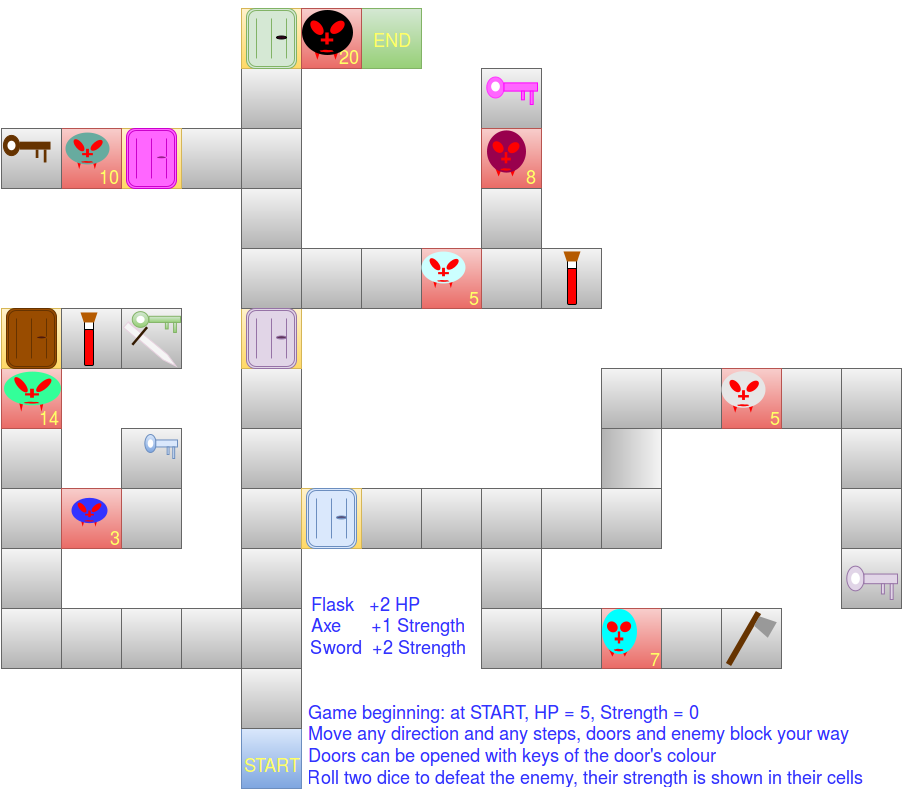
\includegraphics[width=\textwidth]{simpleGameDesign.png}
  \noindent\makebox[\textwidth]{%
  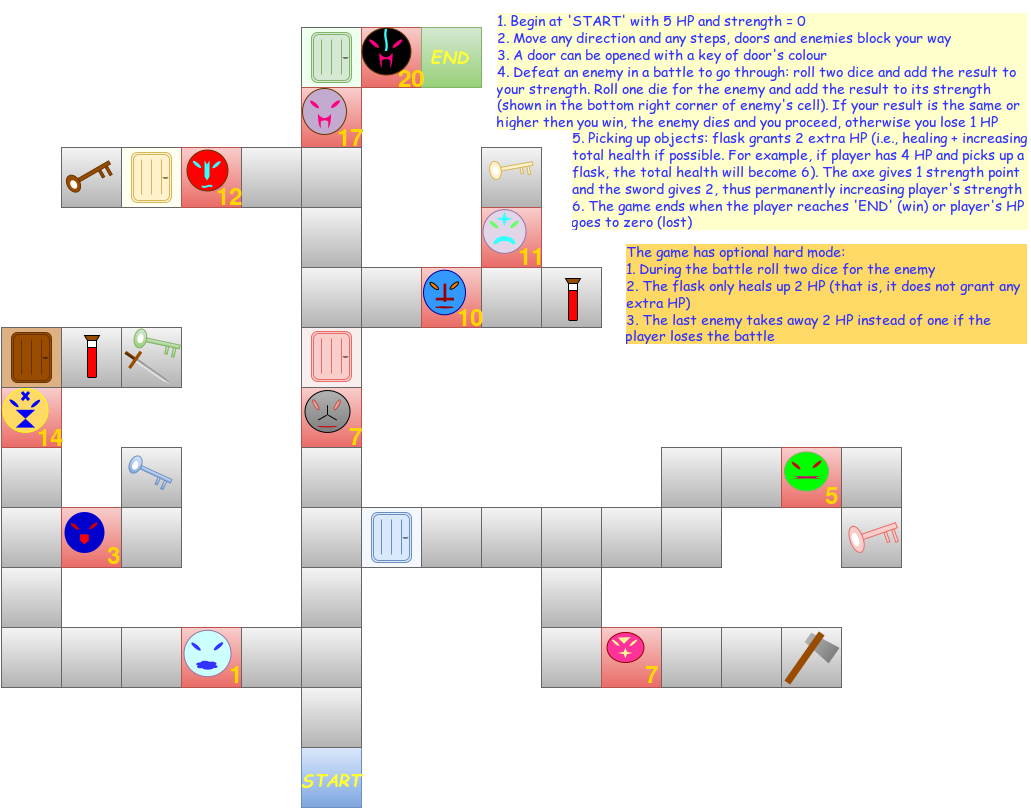
\includegraphics[height=\textheight]{simpleGameDesign2.png}
}
\end{figure}

\end{document}
